\subsection{Relación 1}
\setcounter{ejercicio}{0}

\begin{ejercicio}\label{ej:1.1.1}
    Se considera el problema de encontrar las soluciones reales de la ecuación $x + \nicefrac{1}{2} - 2\sen(\pi x) = 0$ en el intervalo $\left[\nicefrac{1}{2},\nicefrac{3}{2}\right]$.
    \begin{enumerate}
        \item ¿Se puede utilizar el método de bisección para resolver dicho problema tomando $\left[\nicefrac{1}{2},\nicefrac{3}{2}\right]$ como intervalo inicial? ¿Por qué? En caso afirmativo, calcule las tres primeras iteraciones de dicho método.
        
        Definimos la función siguiente:
        \Func{f}{\left[\nicefrac{1}{2},\nicefrac{3}{2}\right]}{\bb{R}}{x}{x + \nicefrac{1}{2} - 2\sen(\pi x)}

        Sabemos que $f\in C^{\infty}\left(\left[\frac{1}{2},\frac{3}{2}\right]\right)$, y además:
        \begin{align*}
            f\left(\frac{1}{2}\right)&=1-2\sen\left(\frac{\pi}{2}\right)=-1<0\\
            f\left(\frac{3}{2}\right)&=2-2\sen\left(\frac{3\pi}{2}\right)=4>0
        \end{align*}

        Por lo tanto, por el teorema de Bolzano, existe al menos una raíz en el intervalo $\left[\nicefrac{1}{2},\nicefrac{3}{2}\right]$. Por tanto, podemos aplicar el método de bisección.
        Calculamos las tres primeras iteraciones:
        \begin{equation*}
            \begin{array}{c|cccc}
                n & a_n & b_n & x_n & f(x_n)\\
                \hline
                0 & 0.5 & 1.5 & 1 & 1.5\\
                1 & 0.5 & 1 & 0.75 & -0.1642\\
                2 & 0.75 & 1 & 0.875 & 0.6096\\
                3 & 0.75 & 0.875 & 0.8125
            \end{array}
        \end{equation*}
        \item Halle una cota del error que se comete si consideramos la última de las iteraciones del apartado anterior como el valor de la solución del problema dado.
        
        

        Tenemos que:
        \begin{equation*}
            |e_3| \leq \dfrac{1}{2^{4}}\left(\dfrac{3}{2}-\dfrac{1}{2}\right)=\dfrac{1}{16}=0.0625
        \end{equation*}
        \item ¿Cuántas iteraciones del método de bisección son necesarias para garantizar un error menor que $10^{-5}$?
        
        Para garantizar un error menor que $10^{-5}$ necesitamos que:
        \begin{align*}
            |e_n| \leq \dfrac{1}{2^{n+1}}\leq 10^{-5} \iff 10^5\leq 2^{n+1}\iff n\geq \log_2(10^5)-1\approx 15.6096
        \end{align*}

        Como $n$ debe ser entero, necesitamos al menos 16 iteraciones.
    \end{enumerate}
\end{ejercicio}

\begin{ejercicio}\label{ej:1.1.2}
    Se quiere calcular el inverso de un número real $c > 0$ sin efectuar divisiones. Para ello, se elige un valor $x_0 > 0$ y se considera el método iterativo dado por $x_{n+1} = x_n(2 - cx_n)$, $n \geq 0$.
    \begin{enumerate}
        \item Demuestre que la sucesión generada por dicho método converge a $\nicefrac{1}{c}$ si y sólo si $0 < x_0 < \nicefrac{2}{c}$.
        \begin{observacion}
            Comience demostrando por inducción que $r_n = r^{2^n}_0$ $\forall n \geq 0$ siendo $r_n = 1 - cx_n$.
        \end{observacion} 

        Demostramos por inducción dicha observación:
        \begin{itemize}
            \item \ul{Caso base}: $n=0$.
            \begin{equation*}
                r_0^{2^0}=r_0^1=r_0
            \end{equation*}

            \item \ul{Paso inductivo}: Supongamos que $r_n=r_0^{2^n}$.
            \begin{align*}
                r_0^{2^{n+1}}&=\left(r_0^{2^n}\right)^2=r_n^2=\left(1-cx_n\right)^2
                =1-2cx_n+c^2x_n^2
                = 1-cx_n\left(2-cx_n\right)
                =\\&= 1-cx_{n+1}=r_{n+1}
            \end{align*}

            Por lo tanto, $r_n=r_0^{2^n}$ para todo $n\geq 0$.
            Por la suma geométrica, tenemos que:
            \begin{align*}
                \{x_n\}\ \text{es convergente} &\iff \{r_n\}\ \text{es convergente} \iff\\&\iff |r_0|<1 \iff |1-cx_0|<1 \iff 0<cx_0<2\iff\\&\iff 0<x_0<\frac{2}{c}
            \end{align*}

            En el caso de que sea convergente, por la unicidad del límite, se tiene que:
            \begin{align*}
                1-c\lim_{n\to \infty}x_n
                =\lim_{n\to \infty} \left(1-cx_n\right)=
                \lim_{n\to \infty}r_n=0
                \Longrightarrow
                \lim_{n\to \infty}x_n = \frac{1}{c}
            \end{align*}
        \end{itemize}
        \item Demuestre que la convergencia referida en el apartado anterior es al menos cuadrática. ¿Cuál es la constante asintótica del error?
        
        Definimos la función siguiente:
        \Func{g}{\left[0,\frac{2}{c}\right]}{\bb{R}}{x}{x(2-cx)}

        Tenemos que:
        \begin{equation*}
            g\left(\frac{1}{c}\right)=\frac{1}{c}\left(2-\frac{c}{c}\right)=\frac{1}{c}
        \end{equation*}

        Calculamos las dos primeras derivadas de $g$:
        \begin{align*}
            g'(x)&=2-cx-cx=2(1-cx)\\
            g''(x)&=-2c
        \end{align*}

        Evaluando en el punto fijo de $g$:
        \begin{align*}
            g'\left(\frac{1}{c}\right)&=2(1-c\cdot\frac{1}{c})=2(1-1)=0\\
            g''\left(\frac{1}{c}\right)&=-2c\neq 0
        \end{align*}

        Por tanto, el método iterativo $x_{n+1}=g(x_n)$ tiene orden de convergencia cuadrático, con constante asintótica del error:
        \begin{equation*}
            C=\frac{1}{2}\cdot 2c=c
        \end{equation*}
        \item Compruebe que el método iterativo propuesto es el método de Newton-Raphson aplicado a una cierta ecuación $f(x) = 0$ cuya única raíz es $\nicefrac{1}{c}$.
        
        Sea $f$ la función que buscamos. Entonces:
        \begin{equation*}
            x-\dfrac{f(x)}{f'(x)} = g(x)=x(2-cx)
            \Longrightarrow
            \dfrac{f(x)}{f'(x)}=x-2x+cx^2=cx^2-x
        \end{equation*}

        Podríamos intentar resolver dicha ecuación diferencial en variables separadas, pero directamente probaremos con varias funciones que tienen a $\nicefrac{1}{c}$ como raíz, y veamos con cuál se da lo anterior.
        \begin{itemize}
            \item $f(x)=x-\nicefrac{1}{c}$.
            \begin{align*}
                f'(x)&=1\\
                \dfrac{f(x)}{f'(x)}&=f(x)=x-\nicefrac{1}{c}
            \end{align*}

            Por tanto, vemos que esta no es la función que buscamos.

            \item $f(x)=c-\nicefrac{1}{x}$.
            \begin{align*}
                f'(x)&=\nicefrac{1}{x^2}\\
                \dfrac{f(x)}{f'(x)}&=cx^2-x
            \end{align*}

            Por tanto, esta es la función que buscamos.
        \end{itemize}

        Por tanto, el método iterativo propuesto es el método de Newton-Raphson aplicado a la ecuación $f(x)=0$ con $f(x)=c-\nicefrac{1}{x}$, cuya única raíz es $\nicefrac{1}{c}$.
    \end{enumerate}
\end{ejercicio}


\begin{ejercicio}\label{ej:1.1.3}
    Demuestre que la ecuación $x^3 - 2x^2 - 5 = 0$ tiene una única solución en el intervalo $[1, 4]$. Elija una semilla $x_0$ que permita hallar, usando el método de Newton-Raphson, una aproximación a dicha solución y justifique dicha elección. Calcule las dos primeras iteraciones.

    Definimos la función siguiente:
    \Func{f}{[1,4]}{\bb{R}}{x}{x^3-2x^2-5}

    Sabemos que $f\in C^{\infty}([1,4])$, y además:
    \begin{align*}
        f(1)&=1-2-5=-6<0\\
        f(4)&=64-32-5=27>0
    \end{align*}

    Por lo tanto, por el teorema de Bolzano, existe al menos una raíz en el intervalo $[1,4]$. Veamos ahora que esta es única:
    \begin{equation*}
        f'(x)=3x^2-4x=x(3x-4)=0\iff x\in \left\{0,\frac{4}{3}\right\}
    \end{equation*}
    \begin{itemize}
        \item Si $x\in[1,\nicefrac{4}{3}]$, entonces $f'(x)\leq 0$.
        
        Como $f(1)<0$ y $f$ es continua, entonces $f$ no tiene raíces reales en $[1,\frac{4}{3}]$.
        \item Si $x\in[\nicefrac{4}{3},4]$, entonces $f'(x)\geq 0$.
        
        Como $f(\nicefrac{4}{3})<0$ y $f$ en este intervalo es inyectiva, entonces, de tener una raíz, sería única.
    \end{itemize}

    Por tanto, la ecuación $x^3-2x^2-5=0$ tiene una única solución en el intervalo $[\nicefrac{4}{3},4]$. Buscamos ahora demostrar la convergencia de Newton-Raphson:
    \begin{enumerate}
        \item $f(\nicefrac{4}{3})f(4)<0$.
        \item $f'(x)$ no se anula en $]\nicefrac{4}{3},4]$.
        \item $f''(x)=6x-4$ no se anula en $]\nicefrac{4}{3},4]$.
        \item Comprobemos que tomar $x_0=4$ sirve para garantizar la convergencia.
        \begin{equation*}
            f(4)f''(4)=27\cdot 20=540>0
        \end{equation*}
    \end{enumerate}

    Por tanto, podemos aplicar el método de Newton-Raphson empleando como semilla $x_0=4$. Calculamos las dos primeras iteraciones:
    \begin{equation*}
        \begin{array}{c|c}
            n & x_n\\
            \hline
            0 & 4\\
            1 & 3.15625\\
            2 & 2.77860
        \end{array}
    \end{equation*}
\end{ejercicio}


\begin{ejercicio}\label{ej:1.1.4}
    Deduzca la fórmula para el cálculo de las iteraciones del método de la secante a partir de su interpretación gráfica.

    Dados dos puntos $(x_n, f(x_n))$ y $(x_{n-1}, f(x_{n-1}))$, la recta secante que pasa por ellos es:
    \begin{equation*}
        \dfrac{y-f(x_{n})}{x-x_{n}}=\dfrac{f(x_n)-f(x_{n-1})}{x_n-x_{n-1}}
    \end{equation*}

    El punto de corte de la recta secante con el eje $x$ es:
    \begin{align*}
        \dfrac{0-f(x_{n})}{x-x_{n}}&=\dfrac{f(x_n)-f(x_{n-1})}{x_n-x_{n-1}}\\
        x-x_{n}&=-f(x_{n})\dfrac{x_n-x_{n-1}}{f(x_n)-f(x_{n-1})}\\
        x&=x_{n}-f(x_{n})\dfrac{x_n-x_{n-1}}{f(x_n)-f(x_{n-1})}
    \end{align*}

    Por tanto, denotamos por $x_{n+1}$ a dicho punto de corte, y obtenemos la fórmula del método de la secante:
    \begin{equation*}
        x_{n+1}=x_n-f(x_n)\dfrac{x_n-x_{n-1}}{f(x_n)-f(x_{n-1})}
    \end{equation*}
\end{ejercicio}


\begin{ejercicio}\label{ej:1.1.5}
    Dada la ecuación $x - \nicefrac{1}{2}\cos(x) = 0$, se pide:
    \begin{enumerate}
        \item Demuestre que tiene una única solución real en el intervalo $\left[0,\nicefrac{\pi}{2}\right]$.
        
        Definimos la función siguiente:
        \Func{f}{[0,\nicefrac{\pi}{2}]}{\bb{R}}{x}{x-\nicefrac{1}{2}\cos(x)}

        Sabemos que $f\in C^{\infty}([0,\nicefrac{\pi}{2}])$. Estudiemos su monotonía:
        \begin{align*}
            f'(x)=1+\nicefrac{1}{2}\sen(x)>0\ \forall x\in[0,\nicefrac{\pi}{2}]
        \end{align*}
        Por tanto, $f$ es inyectiva. Veamos ahora que tiene una única raíz:
        \begin{align*}
            f(0)&=0-\nicefrac{1}{2}\cos(0)=\nicefrac{-1}{2}<0\\
            f\left(\nicefrac{\pi}{2}\right)&=\nicefrac{\pi}{2}>0
        \end{align*}
        Por el teorema de Bolzano, existe al menos una raíz en el intervalo $[0,\nicefrac{\pi}{2}]$. Por la inyectividad de $f$, esta raíz es única.
        
        \item\label{ej:1.1.5b}
        Describa un método de iteración funcional, distinto del método de Newton-Raphson, que permita aproximar dicha solución, razonando la respuesta.\\

        Definimos la función siguiente:
        \Func{g}{[0,\nicefrac{\pi}{2}]}{\bb{R}}{x}{\nicefrac{1}{2}\cos(x)}

        Veamos que las raíces de $f$ son los puntos fijos de $g$:
        \begin{align*}
            f(x)=0&\iff x=\nicefrac{1}{2}\cos(x)\iff x=g(x)
        \end{align*}

        Comprobamos que la función será contractiva en un entorno del punto fijo $s$:
        \begin{equation*}
            |g'(x)|=\nicefrac{1}{2}|\sen(x)|\leq \nicefrac{1}{2}<1
        \end{equation*}

        Por tanto, podemos aplicar el método de iteración funcional $x_{n+1}=g(x_n)$ para aproximar la solución de la ecuación $x-\nicefrac{1}{2}\cos(x)=0$ partiendo de una semilla $x_0$ suficientemente próxima a la solución. Para especificar cuánto es ``suficientemente próxima'', veamos que $g\left([0,\nicefrac{\pi}{2}]\right)\subset [0,\nicefrac{\pi}{2}]$. Sea $x\in[0,\nicefrac{\pi}{2}]$, y entonces:
        \begin{equation*}
            0\leq g(x)=\frac{1}{2}\cos(x)\leq \frac{1}{2}<\frac{\pi}{2}
        \end{equation*}

        Por tanto, $g$ es una contracción en $[0,\nicefrac{\pi}{2}]$, y por tanto, podemos aplicar el método de iteración funcional para aproximar la solución de la ecuación $x-\nicefrac{1}{2}\cos(x)=0$.

        
        \item Realice las dos primeras iteraciones del método descrito en el apartado anterior.
        \begin{equation*}
            \begin{array}{c|c}
                n & x_n\\
                \hline
                0 & \nicefrac{\pi}{4}\approx 0.785398\\
                1 & 0.3535533\\
                2 & 0.4690742\\
                3 & 0.4459936
            \end{array}
        \end{equation*}
        \item ¿Cuántas iteraciones es preciso realizar para garantizar un error menor que $10^{-2}$ en el método dado en el apartado \ref{ej:1.1.5b}?
        
        Para garantizar un error menor que $10^{-2}$ necesitamos que:
        \begin{align*}
            |e_n|&\leq \dfrac{L^n}{1-L}\cdot |x_{1}-x_0|\leq \frac{1}{2^{n}(1-\nicefrac{1}{2})}\cdot |x_1-x_0|=\frac{0.43199}{2^{n+1}}
            \leq 10^{-2}\iff\\&\iff 2^{n-1}\geq \frac{0.43199}{10^{-2}}= 43.199
            \iff n\geq \log_2(43.199)+1\approx 6.4329
        \end{align*}

        Como $n$ debe ser entero, necesitamos al menos 7 iteraciones.

    \end{enumerate}
\end{ejercicio}

\begin{ejercicio}\label{ej:1.1.6}
    Usando algún resultado sobre convergencia para los métodos de iteración funcional, demuestre el teorema de convergencia local para ceros simples del método de Newton-Raphson.
\end{ejercicio}

\begin{ejercicio}\label{ej:1.1.7}
    Para resolver la ecuación $f(x) = 0$ se considera el método $x_{n+1} = x_n - \nicefrac{f(x_n)}{m}$, donde $m \neq 0$.
    \begin{enumerate}
        \item Interprete gráficamente el cálculo de las iteraciones según dicho método.
        \item ¿Qué condiciones para la función $f$, para la constante $m$ y para el valor inicial $x_0$ asegurarían unicidad de solución y convergencia a dicha solución del método considerado?
    \end{enumerate}
\end{ejercicio}

\begin{ejercicio}\label{ej:1.1.8}
    Localice un intervalo $[a, b]$ en el que se encuentren todas las soluciones reales de la ecuación $2x^4 - 3x^2 + 3x - 4 = 0$, y sepárelas. Tomando $x_0 = -2$ como semilla, calcule las tres primeras iteraciones del método de Newton-Raphson usando el algoritmo de Horner.
\end{ejercicio}

\begin{ejercicio}\label{ej:1.1.9}
    Sea $s = \sqrt{3}$. Para calcular $s$ se considera el método de iteración funcional 
    \begin{equation*}
        x_{n+1} = g(x_n) \quad \text{con} \quad g(x) = ax + \frac{x^3}{3} + bx^2.
    \end{equation*}

    Halle los valores de $a$ y $b$ para que, partiendo de una semilla $x_0$ suficientemente próxima a $s$, se asegure la convergencia al menos cuadrática. Para tales valores, calcule $x_3$ para $x_0 = 1$.
\end{ejercicio}

\begin{ejercicio}\label{ej:1.1.10}
    Se desea aplicar un método iterativo del siguiente tipo para obtener $\sqrt[3]{7}$.
    $$x_{n+1} = p\cdot x_n + q\cdot \nicefrac{7}{x^2_n} + r\cdot \nicefrac{7^2}{x^5_n}$$
    Halle los valores de $p$, $q$, $r$ para que la convergencia local del método sea al menos cúbica. Realice dos iteraciones partiendo de $x_0 = 2$.
\end{ejercicio}

\begin{ejercicio}\label{ej:1.1.11}
    Sea $f(x) = x^5 + x^2 - 1$.
    \begin{enumerate}
        \item ¿Cuántas raíces tiene la ecuación $f(x) = 0$ en el intervalo $[0, 1]$?
        \item Pruebe que el método de iteración funcional
        $$x_{n+1} = g(x_n) = \sqrt[3]{\dfrac{1}{x_n^3+1}}$$
        converge en el intervalo $[0, 1]$ a una raíz de $f(x) = 0$.
        \item Localice todas las raíces reales de $f(x)$.
    \end{enumerate}
\end{ejercicio}

\begin{ejercicio}\label{ej:1.1.12}
    A partir de la gráfica de $y = f(x)$ que se muestra, determine gráficamente las dos aproximaciones siguientes que generan los métodos de Newton-Raphson y de la secante partiendo de las semillas que aparecen en cada caso. Deduzca si hay convergencia y hacia qué solución de $f(x) = 0$.
    \begin{enumerate}
        \item Método de Newton-Raphson: Figura \ref{fig:1.12_1}.
        \item Método de la secante: Figura~\ref{fig:1.12_2}.
    \end{enumerate}
\end{ejercicio}


\begin{figure}
    \centering
    \begin{tikzpicture}
        \begin{axis}[
            axis x line=center,
            axis y line=center,
            xmin=-1,
            xmax=1,
            ymin=-0.5,
            ymax=0.6,
            domain=-0.85:0.9,
            samples=100,
            % No haya ticks
            xtick=\empty,
            ytick=\empty,
        ]
            \addplot[blue, thick] {4*x^4 - 0.5*x^3 - 3*x^2 + 0.3};


            % 0.6, f(0.6)
            \addplot[mark=*] coordinates {(0.6, -0.3696)};

            % x_0 en el punto (0.6, 0)
            \addplot[mark=*] coordinates {(0.6, 0)};
            \node[above] at (axis cs:0.6, 0) {$x_0$};

            % Recta dicontinua que une (0.6, 0) con (0.6, f(0.6))
            \addplot[dashed] coordinates {(0.6, 0) (0.6, -0.3696)};
        \end{axis}
    \end{tikzpicture}
    \caption{Semilla para el método de Newton-Raphson en el Ejercicio \ref{ej:1.1.12}.}
    \label{fig:1.12_1}
\end{figure}



\begin{figure}
    \centering
    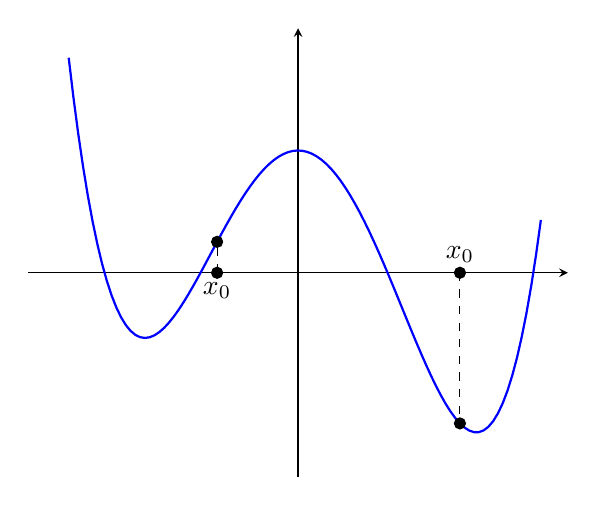
\begin{tikzpicture}
        \begin{axis}[
            axis x line=center,
            axis y line=center,
            xmin=-1,
            xmax=1,
            ymin=-0.5,
            ymax=0.6,
            domain=-0.85:0.9,
            samples=100,
            % No haya ticks
            xtick=\empty,
            ytick=\empty,
        ]
            \addplot[blue, thick] {4*x^4 - 0.5*x^3 - 3*x^2 + 0.3};


            % 0.6, f(0.6)
            \addplot[mark=*] coordinates {(0.6, -0.3696)};

            % x_0 en el punto (0.6, 0)
            \addplot[mark=*] coordinates {(0.6, 0)};
            \node[above] at (axis cs:0.6, 0) {$x_0$};

            % Recta dicontinua que une (0.6, 0) con (0.6, f(0.6))
            \addplot[dashed] coordinates {(0.6, 0) (0.6, -0.3696)};


            % -0.3, f(-0.3)
            \addplot[mark=*] coordinates {(-0.3, 0.0759)};

            % x_0 en el punto (-0.3, 0)
            \addplot[mark=*] coordinates {(-0.3, 0)};
            \node[below] at (axis cs:-0.3, 0) {$x_0$};

            % Recta dicontinua que une (-0.3, 0) con (-0.3, f(-0.3))
            \addplot[dashed] coordinates {(-0.3, 0) (-0.3, 0.0759)};
        \end{axis}
    \end{tikzpicture}
    \caption{Semilla para el método de la Secante en el Ejercicio \ref{ej:1.1.12}.}
    \label{fig:1.12_2}
\end{figure}


\begin{ejercicio}\label{ej:1.1.13}
    Se considera la ecuación $xe^{-x^3} + 1 = 0$ y los métodos de iteración funcional $x_{n+1} = g(x_n)$ dados por las funciones
    \begin{align*}
        g_1(x) &= -e^{\nicefrac{x}{3}}, & g_2(x) &= e^{\nicefrac{x}{3}}, \\
        g_3(x) &= 3\ln(-x), & g_4(x) &= \dfrac{x-e^{\nicefrac{x}{3}}}{2}.
    \end{align*}
    \begin{enumerate}
        \item Encuentre un intervalo de amplitud 1 donde haya una única raíz de la ecuación.
        \item Averigüe cuáles de los métodos propuestos son compatibles con la ecuación dada; es decir, para cuáles de ellos la solución es punto fijo.
        \item De entre los métodos compatibles con la ecuación ¿cuáles son convergentes localmente? Justifique la respuesta.
        \item De entre los métodos convergentes localmente ¿cuál es el más rápido? ¿Por qué?
        \item Para los métodos que hayan resultado divergentes, aplique Steffensen con $x_0 = -0.5$ hasta que dos iteraciones consecutivas disten menos de $10^{-3}$.
    \end{enumerate}
\end{ejercicio}


\begin{ejercicio}\label{ej:1.1.14}
    Supongamos que se modifica el método de bisección cambiando el punto de división del intervalo por el valor $a + \frac{b-a}{3}$ (porque se cree que la solución está más cerca del extremo $a$). ¿Es convergente dicho método? ¿Cuál es la cota del error absoluto después de $n$ iteraciones?
\end{ejercicio}

\begin{ejercicio}\label{ej:1.1.15}
    Demuestre el teorema de convergencia global de los métodos de iteración funcional para sistemas.
    \begin{observacion}
        Generalice al caso $k$-dimensional la demostración del teorema de convergencia global de los métodos de iteración funcional unidimensional.
    \end{observacion}
\end{ejercicio}

\begin{ejercicio}\label{ej:1.1.16}
    Sea $D = \prod\limits_{i=1}^k[a_i, b_i]$ y sea $G : D \to \bb{R}^k$ con $G = (g_1, \ldots, g_k)$ tal que $G \in C^1(D)$. Demuestre que si existe $L \in\left]0, 1\right[$ tal que $\forall i, j = 1, \ldots, k$ se verifique
    \begin{equation*}
        \left\lvert \dfrac{\partial g_i(x)}{\partial x_j} \right\rvert \leq \dfrac{L}{k}\quad \forall x \in D,
    \end{equation*}
    entonces $G$ es contráctil.
    \begin{observacion}
        Considere la norma $\| \cdot \|_1$ o $\| \cdot \|_\infty$.
    \end{observacion}
\end{ejercicio}

\begin{ejercicio}\label{ej:1.1.17}
    Se considera el sistema de ecuaciones
    \begin{align*}
        \dfrac{x^2-y^2}{2}-x + \frac{7}{24} &= 0, \\
        xy - y + \frac{1}{9} &= 0.
    \end{align*}
    \begin{enumerate}
        \item Demuestre que tiene una única solución en el rectángulo $D = [0, 0.4] \times [0, 0.4]$.
        \item Encuentre una sucesión que converja a dicha solución, justificando la respuesta.
        \item Calcule, tomando $x_0 = (0.1, 0.2)$, las dos primeras iteraciones del método de Newton-Raphson para el sistema.
    \end{enumerate}
\end{ejercicio}


\begin{ejercicio}\label{ej:1.1.18}
    Se considera el sistema de ecuaciones
    \begin{align*}
        x - xy &= \nicefrac{1}{16}, \\
        x^2 - y &= \nicefrac{-1}{8}.
    \end{align*}
    \begin{enumerate}
        \item Demuestre que tiene una única solución en el rectángulo $D = [0, \nicefrac{1}{8}] \times [0, \nicefrac{1}{4}]$.
        \item Encuentre una sucesión que converja a dicha solución, justificando la respuesta.
        \item Calcule, tomando $x_0 = (0.1, 0.2)$, las dos primeras iteraciones del método de Newton-Raphson para el sistema.
    \end{enumerate}
\end{ejercicio}